% This file is for the main body, update section heading and add relevant additional sections as required

\section{Star Graphs}

In this section, we consider games on \textit{star graphs}, i.e., bipartite graphs where one of the partitions is a singleton set. We will start with the complete characterization of imputations in the core of these games.\\
% \todo[inline]{Add some intuition, and probably use cases, of star graphs in transportation games.}
\begin{figure}[H]
    \centering
    \begin{tikzpicture}[scale=1.5, every node/.style={inner sep=1pt}]
        \small
        % Nodes
        \node[draw, circle, minimum size=0.45cm] (u) at (0, 2) {$u$};
        \node[draw, circle, minimum size=0.45cm] (v1) at (-3, 0) {$v_1$};
        \node[draw, circle, minimum size=0.45cm] (v2) at (-1, 0) {$v_2$};
        \node[draw, circle, minimum size=0.45cm] (vn) at (2.5, 0) {$v_n$};
        
        % Connecting edges
        \draw (u) -- (v1) node[midway, left] {$w_1$};
        \draw (u) -- (v2) node[midway, left] {$w_2$};
        \draw (u) -- (vn) node[midway, right] {$w_n$};
      
        % Dots
        \path (v2) -- (vn) node[midway, draw=none] {$\cdots$};
    \end{tikzpicture}
    \caption{A star graph $G=(U,V,E)$.}
    \label{fig:general_stars}
\end{figure}
Let us consider a $b$-matching game on a star graph $G=(U,V,E)$ with $U=\{u\}, V=\{v_1,v_2,\ldots, $ $v_n\},$ $E = \{e_i| e_i=(u,v_i), \forall v_i\in V\}$. Let the weight on edges and the capacities on vertices be given by $w:E\rightarrow \mathbb{R}_+$ and $b:U\cup V \rightarrow \mathbb{Z}_+$. We will refer to the agent $u$ as the \textit{central} player and the agents in $V$ as \textit{leaf} players. For ease of notation, let us represent the profit of the central agent by $p_u$ and the leaf agents by $p_i = p_{v_i}$. 


\subsection{Efficient Characterization of the Core}

Before we give a characterization, we will first revisit the notion of \textit{marginal utility} of an agent.
\begin{definition}
    In a game $G=(N,\nu)$, the \textit{marginal untility} of an agent $i \in N$ is the decrease in the total worth of the game with the exclusion of $i$.
\end{definition}

We will use $\mu^G(i)$, or $\mu(i)$ if the game is obvious, to represent the marginal utility of agent $i$. Formally, $$ \mu(i) = \nu(G) - \nu(G\setminus \{i\}) $$


\begin{theorem}
\label{thm:star_core_characterization}
    The core of a $b$-matching game on star graphs is completely characterizable. 
\end{theorem}

\begin{proof}
Consider a $b$-matching game on star graph $G$. The core imputations relate to marginal utilities through the following lemma. 
\begin{lemma}
\label{lem:core_marginal_utility}
    An imputation $p:U\cup V \rightarrow \mathbb{R}_+$ is in the core if and only if no leaf player is paid more than its marginal utility, i.e., 
    $$p_i \leq \nu(G) - \nu(G \setminus \{v_i\})$$
\end{lemma}

\begin{proof}
    It is easy to see that the condition is necessary; For contradiction, assume that some leaf player, say $v_i$, gets paid more than its marginal utility, i.e., $p_i > \nu(G) - \nu(G\setminus \{v_i\}) \iff \nu(G) - p_i < \nu(G\setminus \{v_i\})$. Then, by  a simple substitution as shown below, we can see that the sub-coalition of the rest of the vertices, $(U\cup V) \setminus{\{v_i\}}$, will not get enough profit, and so, the imputation is not in the core.  $$p(G\setminus \{v_i\}) = p(G) - p_i = \nu(G) - p_i < \nu(G\setminus \{v_i\})$$

    To show that the condition is also sufficient, we will first discuss a more general property for the star graphs.

    Define $b$-matching ``sub-games'' on star sub-coalitions $S$ of agents, where $S\subseteq U\cup V, u\in S$. We use $S$ to refer to these sub-games, with the characteristic function given by the max. wt. $b$-matchings within this set of agents. Then, we claim the following.

    \begin{claim}
    \label{cl:marginal_utility}
        In star graphs, the marginal utility of a leaf agent is higher in the sub-games than in the original $b$-matching game.\\
        Formally, let $u,v_i \in S$. Then 
    $\mu^S_i \geq \mu^G_i$ or $$ \nu(S) - \nu(S\setminus \{v_i\}) \geq \nu(G) - \nu(G \setminus \{v_i\}) $$
    \end{claim}
    We first argue that the claim is enough to show that the condition is sufficient: Combining $p_i \leq \nu(G)-\nu(G\setminus \{v_i\})$ and the claim, we get $\forall S: p_i \leq \nu(S\cup \{v_i\}) - \nu(S)$. 
    Adding $p(S)$ on both sides to this inequality and rearranging, we have $\forall S: \nu(S\cup \{v_i\}) - p(S\cup \{v_i\}) \geq \nu(S)-p(S)$. Iteratively adding vertices in $G\setminus S$, this inequality gives $\nu(G)-p(G) \geq \nu(S)-p(S)$. Since $p$ is an imputation, we have that $\nu(G)=p(G)$ and so
    
    $$ \forall S, \quad p(S)\geq \nu(S)$$ 

\end{proof}

\end{proof}

Below, we prove the claim on marginal utilities.
\begin{proof}[Proof of~\Cref{cl:marginal_utility}]
    To show this, we show that the marginal utility decreases in the presence of every additional agent, i.e., $$\forall S \subseteq U \cup V, \quad v, v' \notin S: \quad \nu(S \cup \{v\}) - \nu(S) \geq \nu(S \cup \{v, v'\}) - \nu(S \cup \{v'\})$$By adding elements of $G$ not is $S$ in sequence, this identity proves the claim.


   \begin{figure}[H]
    \centering
    \begin{minipage}{0.48\textwidth}
        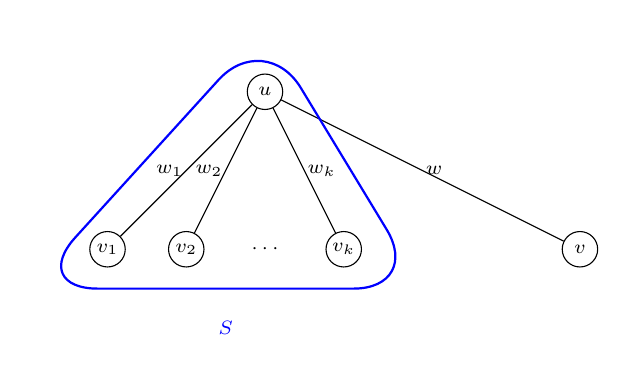
\begin{tikzpicture}[scale=1, every node/.style={inner sep=1pt}]
            \scriptsize
            % Nodes
            \node[draw, circle, minimum size=0.45cm] (u) at (-1, 2) {$u$};
            \node[draw, circle, minimum size=0.45cm] (v1) at (-3, 0) {$v_1$};
            \node[draw, circle, minimum size=0.45cm] (v2) at (-2, 0) {$v_2$};
            \node[draw, circle, minimum size=0.45cm] (vk) at (0, 0) {$v_k$};
            \node[draw, circle, minimum size=0.45cm] (v) at (3, 0) {$v$};

            % Connecting edges
            \draw (u) -- (v1) node[midway, left] {$w_1$};
            \draw (u) -- (v2) node[midway, left] {$w_2$};
            \draw (u) -- (vk) node[midway, right] {$w_k$};
            \draw (u) -- (v) node[midway, right] {$w$};

            % Dots
            \path (v2) -- (vk) node[midway, draw=none] {$\cdots$};

            % Enclosing large circle
           \draw[blue, thick, rounded corners=25pt] 
            (-4, -0.5) -- (1, -0.5) -- (-1, 2.8) -- cycle;
            \node[blue] at (-1.5, -1) {$S$};
        \end{tikzpicture}
    \end{minipage}
    \hfill
    \begin{minipage}{0.48\textwidth}
        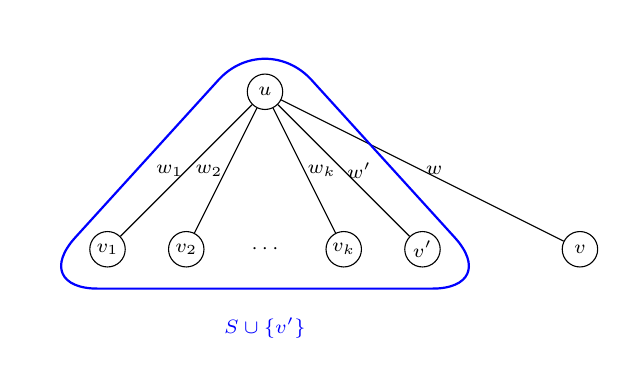
\begin{tikzpicture}[scale=1, every node/.style={inner sep=1pt}]
            \scriptsize
            % Nodes
            \node[draw, circle, minimum size=0.45cm] (u) at (-1, 2) {$u$};
            \node[draw, circle, minimum size=0.45cm] (v1) at (-3, 0) {$v_1$};
            \node[draw, circle, minimum size=0.45cm] (v2) at (-2, 0) {$v_2$};
            \node[draw, circle, minimum size=0.45cm] (vk) at (0, 0) {$v_k$};
            \node[draw, circle, minimum size=0.45cm] (v) at (3, 0) {$v$};
            \node[draw, circle, minimum size=0.45cm] (v') at (1, 0) {$v'$};

            % Connecting edges
            \draw (u) -- (v1) node[midway, left] {$w_1$};
            \draw (u) -- (v2) node[midway, left] {$w_2$};
            \draw (u) -- (vk) node[midway, right] {$w_k$};
            \draw (u) -- (v') node[midway, right] {$w'$};
            \draw (u) -- (v) node[midway, right] {$w$};

            % Dots
            \path (v2) -- (vk) node[midway, draw=none] {$\cdots$};

            % Enclosing large circle
           \draw[blue, thick, rounded corners=25pt] 
            (-4, -0.5) -- (2, -0.5) -- (-1, 2.8) -- cycle;
             \node[blue] at (-1, -1) {$S\cup\{v'\}$};
        \end{tikzpicture}
    \end{minipage}
    \caption{Graphs used in proof of \Cref{cl:marginal_utility}}
    \label{fig:marginal_utility}
\end{figure}


    Consider the graphs in the~\Cref{fig:marginal_utility}. Note that, for star graphs, a max. wt. $b$-matching can just be found by greedily picking the heaviest edges incident on $u$ up to a capacity of $b_{v_i}$ for each $v_i$. 
    
    Let the \textit{weights} of a max. wt. $b$-matching on $S$ be $e_1\geq e_2\geq \ldots \geq e_l$ and that on $S\cup \{v'\}$ be $f_1\geq f_2\geq \ldots \geq f_m$, where $m,l \leq b_u$. Since every edge available in $S$ is also available in $S\cup \{v'\}$, we have $l\leq m$. Let us extend the sequence $e_1\geq e_2\geq \ldots $ up to $m$ terms by adding zeros at the end. As the algorithm is greedy, we also have that $$\forall i\in \{1,2,\ldots,m\} , \quad e_i\leq f_i$$Now bring the vertex $v$ into the graph $S\cup \{v'\}$. Let it replace edges $f_{i_1} \geq f_{i_2} \geq \ldots \geq f_{i_t}$ with the edge $(u,v)$ of weight $w$ to get the max. wt. $b$-matching of $S\cup \{v,v'\}$. Then, replacing the corresponding edges $e_{i_1} \geq e_{i_2} \geq \ldots \geq  e_{i_t}$ with the edge $(u,v)$ will give us a valid $b$-matching in the graph $S\cup \{v\}$. And so, $$\nu(S\cup \{v,v'\}) - \nu(S\cup \{v'\}) = \sum_{j=i}^{t}(w-f_{i_j}) \leq \sum_{j=i}^{t}(w-e_{i_j}) \leq \nu(S\cup \{v\}) - \nu(S)$$ The first inequality comes from $e_i\leq f_i$ and the second inequality is true as the matching obtained by replacing edges $e_{i_1}, e_{i_2},\ldots, e_{i_t}$ with the edge $(u,v)$ need not be the max. wt. $b$-matching in $S\cup \{v\}$. This completes the claim. 
    
    
 \end{proof} 


\begin{corollary}
\label{cr:imputation_star}
There exists a polynomial time algorithm to decide if an imputation is in the core of $b$-matching games on star graphs.
\end{corollary}
%\todo{theorem 3 and 1 are similar ...}

\begin{proof}
    From~\Cref{lem:core_marginal_utility}, we only need to compute the marginal utilities of each leaf agent. And marginal utilities of each leaf agent $v_i$ can be computed just by solving for the max. wt. $b$-matching in $G$ and $G\setminus\{v_i\}$. \cite{Schrijver_book} details a strongly polynomial algorithm to compute the max. wt. $b$-matching in a graph. Combining the above, we get a strongly polynomial time algorithm to decide if an imputation is in the core of $b$-matching games on star graphs.
\end{proof}

\subsection{Unstable Coalitions under General Profit Shares}

\begin{definition}
    Given a cooperative game $G=(N,\nu)$ and a profit share $p$, an \textit{unstable coalition} $S\subseteq N$ is a set of agents who receive a profit less than their worth, i.e., $p(S)<\nu(S)$.
\end{definition}

Under this profit share, such sub-coalitions will break away from the grand coalition and hence cause instability. Given a profit share, our goal is to decide if such unstable sub-coalitions exist. The below theorem shows that the task is intractable.

\begin{theorem}
\label{thm:profit_share_for_star}
    Given a $b$-matching game on a star graph and a profit share, deciding if there exists an unstable sub-coalition is NP-complete.
    % \todo{Think about the definition of core for the profit share}
\end{theorem}

%\begin{theorem}
%    There is a pseudo-polynomial time algorithm to decide if a profit share is in the core of $b$-matching games on star graphs.
%\end{theorem}


\begin{proof}

%\todo[inline]{Replace all capital v and capital p to small letters. Ensure the notation is consistent with the notation and terms defined in the preliminaries.}

In this section, we will use the reduction from the \textsc{0-1 Knapsack Problem} which is stated as follows:
\begin{center}
\begin{tabular}{|>{\centering\arraybackslash}m{2cm}|m{10cm}|}
\hline
\multicolumn{2}{|c|}{\textsc{0-1 Knapsack Problem}} \\ \hline
\textbf{Instance:} & A set of $ n $ items $ \{1, 2, \dots, n\} $, each with a weight $ c_i \in \mathbb{N}$ and a value $ a_i \in \mathbb{N} $, and a knapsack with a maximum weight capacity $ C \in \mathbb{N} $ and a goal value $A \in \mathbb{N}$. \\ \hline
\textbf{Question:} & Is there a collection of items $ S \subseteq \{1, 2, \dots, n\} $ such that the total weight $ \sum_{i \in S} c_i \leq C $ and the total value $ \sum_{i \in S} a_i > A$ \\ \hline
\end{tabular}
\end{center}
Consider the following star graph $G^*$.
\begin{figure}[H]
    \centering
    \begin{tikzpicture}[scale=1.5, every node/.style={inner sep=1pt}]
        \small
        % Nodes
        \node[draw, circle, minimum size=0.45cm] (u) at (0, 2) {$u$};
        \node[draw, circle, minimum size=0.45cm] (v1) at (-3, 0) {$v_1$};
        \node[draw, circle, minimum size=0.45cm] (v2) at (-1, 0) {$v_2$};
        \node[draw, circle, minimum size=0.45cm] (vn) at (2.5, 0) {$v_n$};
        
        % Connecting edges
        \draw (u) -- (v1) node[midway, left] {$w_1$};
        \draw (u) -- (v2) node[midway, left] {$w_2$};
        \draw (u) -- (vn) node[midway, right] {$w_n$};
      
        % Dots
        \path (v2) -- (vn) node[midway, draw=none] {$\cdots$};
    \end{tikzpicture}
    \caption{Graph $G^*$ used in proof of~\Cref{thm:profit_share_for_star}}
    \label{fig:star}
\end{figure}
% \begin{center}
% \begin{tikzpicture}[scale=1.5, every node/.style={inner sep=1pt}]

% % Nodes
% \node[draw, circle, minimum size=0.6cm] (u) at (0, 2) {$u$};
% \node[draw, circle, minimum size=0.6cm] (v1) at (-2, 0) {$v_1$};
% \node[draw, circle, minimum size=0.6cm] (v2) at (-1, 0) {$v_2$};
% \node[draw, circle, minimum size=0.6cm] (vn) at (2, 0) {$v_n$};

% % Connecting edges
% \draw (u) -- (v1) node[midway, above left] {$w_1$};
% \draw (u) -- (v2) node[midway, above left] {$w_2$};
% \draw (u) -- (vn) node[midway, above right] {$w_n$};

% % Dots
% \path (v2) -- (vn) node[midway, draw=none] {$\cdots$};

% \end{tikzpicture}
% \end{center}


% we are going to prove that deciding if a profit share satisfies all core constraints even for star graphs is co-Np-hard. In this regard, we use a reduction from KNApSACK pROBLEM. 


%Let there be $ n $ items, where the $ i $-th item has value $ a_i $ and weight $ c_i $. The goal is to decide if a subset $ S $ of items satisfies:
%$
%\sum_{i \in S} c_i \leq C \quad \text{and} \quad \sum_{i \in S} a_i > A.
%$

Let $G^*=(U^*,V^*,E^*)$ such that $U^*= \{u\} , V^*=\{v_1,v_2, \ldots,$ $ v_n\}, E^*= \{(u,v_1),(u,v_2), \dots, (u,v_n)\}$. Represent $w: E^* \rightarrow \mathbb{R}_+$, $b: U^*\cup V^* \rightarrow \mathbb{Z}_+$ and $p: U^*\cup V^* \rightarrow \mathbb{R}_+$ as follows.

$$b_i:= b(v_i), \quad w_i:= w((u,v_i)) ,   \quad b_u:=b(u) , \quad p_i:= p(v_i), \quad p_u:=p(u)$$

Construct the instance based on knapsack instance as follows:
$
b_i = c_i, \quad w_i = a_i + 1, \quad p_i = -a_i + c_i(a_i + 1),\quad b_u= C, \quad p_u= A.
$
Let $S \subseteq U^*\cup V^*$ be a sub-coalition then: 
%and $v_i \in S$ be an agent that is not fully matched in a max. wt. $b$-matching in $S$. Then:
\begin{lemma}
\label{lem:fully_matched_in_star}
If $ v_i \in S $ and $ v_i $ is not fully matched in a max. wt.$ b $-matching in $ S $, then:
$
\nu(S) - p(S) < \nu(S \setminus \{v_i\}) - p(S \setminus \{v_i\}).
$

\end{lemma}

\begin{proof}
Removing $ v_i $ decreases $ p $ by $ p_i $, and as $v_i$ is not fully matched it decreases $ v $ by at most $ (b_i - 1)w_i $ Thus,
$
\nu(S) - p(S) \text{ increases by at least } p_i - (b_i - 1)w_i,
$
which simplifies to $ 1 $. Hence, $ \nu(S) - p(S)$ increases with the addition of $v_i$.

\end{proof}
\begin{corollary}
\label{cor:fully_matched}
    If $S\subseteq U^*\cup V^*$ is a sub-coalition that maximizes $\nu(S) - p(S)$ then every leaf player of $S$ must be fully matched in all max. wt. $b$-matching in $S$.
\end{corollary}
 
We want to check whether all sub-coalitions $S \subseteq U^*\cup V^*$ satisfy $\nu(S) - p(S) \leq 0$. This is true if the condition holds for all sub-coalitions $S$ that maximize the value of $\nu(S) - p(S)$. \Cref{cor:fully_matched} implies that such coalitions must fully match all their leaf players in their max. wt. $b$-matchings. So let us compute the values of $p(S)$ and $\nu(S)$ for these sets.

\begin{lemma}
    \label{lem:value_in_star}
    Assume that in a max. wt. $b$-matching on a sub-coalition of agents $S$, every vertex in $S \cap V^*$ is fully matched. Then the value of this subset is $\sum_{i \in S\cap v} a_i - A$. 
\end{lemma}
%\subsection{Computing the value}
%Assume that in a max. wt. $b$-matching on $S$ every vertices in $S \cap V$ are fully matched. The value of this subset is 
%$
%\nu(S)= \sum_{i \in S\cap v} b_iw_i
%$
%So:
%$
%\nu(S) - p(S) = (\sum_{i \in S\cap v} b_i w_i) - (\sum_{i \in S\cap v} p_i) - p_u.
%$

%Substituting the values:
%$
%\nu(S) - p(S) = \sum_{i \in S\cap v} c_i(a_i + 1) - \sum_{i \in S\cap v} (c_i(a_i + 1) - a_i) - A,
%$
%Which simplifies to:
%$
%\nu(S) - p(S) = \sum_{i \in S\cap v} a_i - A.
%$
\begin{proof}
All leaf vertices are fully matched so for each leaf vertex $v_i\in S$ it increases the value of $S$ by $b_iw_i$ so:
\begin{align*}
\nu(S) & = \sum_{i \in S \cap v} b_i w_i \\
\nu(S) - p(S) & = \sum_{i \in S \cap v} b_i w_i - \bigg(\sum_{i \in S \cap v} p_i + p_u \bigg) \\
 & = \sum_{i \in S \cap v} c_i (a_i + 1) - \bigg(\sum_{i \in S \cap v} (c_i (a_i + 1) - a_i) + A\bigg) \\
 & = \sum_{i \in S \cap v} a_i - A
\end{align*}
 \end{proof}
If there is a sub-coalition of agents $S$ such that $ \nu(S) - p(S) > 0 $, then we have a collection of items in \textsc{0-1 Knapsack Problem} such that the sum of their values is greater than $A$ and the sum of their weights does not exceed the capacity $C$ because the corresponding sub-coalition of this collection makes a valid $b$-matching, so it is satisfying the knapsack constraints. Conversely, any subset $ S' $ satisfying the knapsack constraints corresponds to an unstable coalition$ S $. So the reduction from \textsc{0-1 Knapsack Problem} is complete.
\end{proof}


